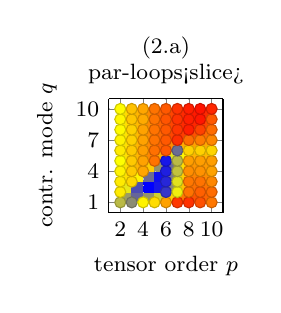
\begin{tikzpicture}
\begin{axis}
[
width=0.25\textwidth,
height=0.25\textwidth,
style={font=\footnotesize},
grid=major,
grid style={dotted},
align=center,
xlabel={tensor order $p$},
ylabel={contr. mode $q$},
title={(2.a)\\\tss{par-loops<slice>}}, %  ompfor<slice>, asymmetric, row-major
title style={yshift=-1ex,},
scaled ticks=false,
zlabel={GFlops/core},
view={0}{90}, 
%view={-45}{45}, 
ytick={1,4,7,10},
xtick={2,4,6,8,10},
xmin=1, xmax=11,
ymin=0, ymax=11,
try min ticks=8,
zmin=10, zmax=50,
point meta min=10, point meta max=50,
colormap/hot, 
samples=50,
]
\addplot3[contour filled={number=100},scatter,shader=flat,samples=50]
coordinates{

(2.000,1.000,19.650) (2.000,2.000,25.593) (2.000,3.000,25.477) (2.000,4.000,24.532) (2.000,5.000,23.459) (2.000,6.000,25.371) (2.000,7.000,24.466) (2.000,8.000,23.636) (2.000,9.000,24.244) (2.000,10.000,23.826) 

(3.000,1.000,17.506) (3.000,2.000,1.820) (3.000,3.000,27.267) (3.000,4.000,28.905) (3.000,5.000,29.095) (3.000,6.000,29.128) (3.000,7.000,28.026) (3.000,8.000,28.218) (3.000,9.000,29.562) (3.000,10.000,29.604) 

(4.000,1.000,24.742) (4.000,2.000,3.508) (4.000,3.000,3.297) (4.000,4.000,32.708) (4.000,5.000,33.191) (4.000,6.000,33.338) (4.000,7.000,33.041) (4.000,8.000,33.130) (4.000,9.000,32.240) (4.000,10.000,32.751) 

(5.000,1.000,27.194) (5.000,2.000,6.860) (5.000,3.000,6.423) (5.000,4.000,6.309) (5.000,5.000,37.825) (5.000,6.000,38.118) (5.000,7.000,37.656) (5.000,8.000,37.722) (5.000,9.000,37.817) (5.000,10.000,37.949) 

(6.000,1.000,32.992) (6.000,2.000,13.034) (6.000,3.000,12.075) (6.000,4.000,11.844) (6.000,5.000,11.520) (6.000,6.000,40.727) (6.000,7.000,40.716) (6.000,8.000,40.523) (6.000,9.000,40.809) (6.000,10.000,40.579) 

(7.000,1.000,43.928) (7.000,2.000,22.640) (7.000,3.000,21.779) (7.000,4.000,20.140) (7.000,5.000,19.765) (7.000,6.000,15.904) (7.000,7.000,44.803) (7.000,8.000,44.344) (7.000,9.000,44.595) (7.000,10.000,44.527) 

(8.000,1.000,44.587) (8.000,2.000,37.971) (8.000,3.000,37.286) (8.000,4.000,35.009) (8.000,5.000,33.488) (8.000,6.000,28.360) (8.000,7.000,38.637) (8.000,8.000,46.575) (8.000,9.000,46.586) (8.000,10.000,46.416) 

(9.000,1.000,41.437) (9.000,2.000,39.862) (9.000,3.000,37.652) (9.000,4.000,34.468) (9.000,5.000,33.392) (9.000,6.000,28.217) (9.000,7.000,37.134) (9.000,8.000,43.121) (9.000,9.000,47.532) (9.000,10.000,47.674) 

(10.000,1.000,37.265) (10.000,2.000,38.454) (10.000,3.000,35.607) (10.000,4.000,33.144) (10.000,5.000,33.530) (10.000,6.000,27.899) (10.000,7.000,35.921) (10.000,8.000,38.708) (10.000,9.000,40.450) (10.000,10.000,45.687) 


};
\end{axis}
\end{tikzpicture}
\hfill
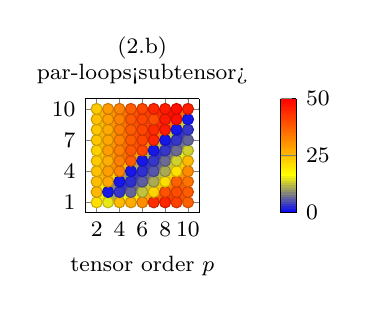
\begin{tikzpicture}
\begin{axis}
[
width=0.25\textwidth,
height=0.25\textwidth,
style={font=\footnotesize},
grid=major,
grid style={dotted},
align=center,
xlabel={tensor order $p$},
%ylabel={contr. mode (q)},
title={(2.b)\\\tss{par-loops<subtensor>}}, %  ompfor<subtensor>, asymmetric, row-major
title style={yshift=-1ex},
scaled ticks=false,
zlabel={GFlops},
view={0}{90}, 
ytick={1,4,7,10},
xtick={2,4,6,8,10},
xmin=1, xmax=11,
ymin=0, ymax=11,
try min ticks=8,
zmin=0, zmax=50,
point meta min=0, point meta max=50,
colormap/hot, 
samples=50,
colorbar sampled,
colorbar/width=0.2cm,
colorbar style={
point meta min=0, point meta max=50,
samples=50,
font=\footnotesize,
ytick={0,25,50},
yticklabels={0,25,50},
%title={\scriptsize Gflops},
%ylabel={\scriptsize Gflops},
}
]
\addplot3[contour filled={number=100},scatter,shader=flat,samples=50]
coordinates{

(2.000,1.000,20.786) (2.000,2.000,25.568) (2.000,3.000,25.388) (2.000,4.000,24.697) (2.000,5.000,23.655) (2.000,6.000,22.860) (2.000,7.000,24.266) (2.000,8.000,24.114) (2.000,9.000,24.538) (2.000,10.000,23.903) 

(3.000,1.000,15.071) (3.000,2.000,1.820) (3.000,3.000,28.071) (3.000,4.000,29.205) (3.000,5.000,27.247) (3.000,6.000,29.424) (3.000,7.000,28.184) (3.000,8.000,27.829) (3.000,9.000,28.913) (3.000,10.000,29.770) 

(4.000,1.000,25.498) (4.000,2.000,3.531) (4.000,3.000,1.770) (4.000,4.000,32.802) (4.000,5.000,33.055) (4.000,6.000,33.292) (4.000,7.000,32.767) (4.000,8.000,33.111) (4.000,9.000,32.563) (4.000,10.000,32.658) 

(5.000,1.000,27.092) (5.000,2.000,6.861) (5.000,3.000,3.419) (5.000,4.000,1.722) (5.000,5.000,37.810) (5.000,6.000,38.077) (5.000,7.000,37.992) (5.000,8.000,37.737) (5.000,9.000,38.044) (5.000,10.000,37.944) 

(6.000,1.000,31.377) (6.000,2.000,12.939) (6.000,3.000,6.475) (6.000,4.000,3.202) (6.000,5.000,1.811) (6.000,6.000,40.597) (6.000,7.000,40.787) (6.000,8.000,40.527) (6.000,9.000,40.684) (6.000,10.000,40.620) 

(7.000,1.000,43.989) (7.000,2.000,22.205) (7.000,3.000,11.241) (7.000,4.000,5.603) (7.000,5.000,3.581) (7.000,6.000,1.801) (7.000,7.000,44.783) (7.000,8.000,44.412) (7.000,9.000,39.607) (7.000,10.000,44.512) 

(8.000,1.000,44.651) (8.000,2.000,39.267) (8.000,3.000,21.378) (8.000,4.000,11.051) (8.000,5.000,7.029) (8.000,6.000,3.572) (8.000,7.000,1.803) (8.000,8.000,46.461) (8.000,9.000,46.447) (8.000,10.000,46.428) 

(9.000,1.000,41.190) (9.000,2.000,39.830) (9.000,3.000,37.237) (9.000,4.000,20.972) (9.000,5.000,13.844) (9.000,6.000,7.057) (9.000,7.000,3.540) (9.000,8.000,1.788) (9.000,9.000,47.565) (9.000,10.000,47.669) 

(10.000,1.000,37.060) (10.000,2.000,37.835) (10.000,3.000,34.503) (10.000,4.000,31.880) (10.000,5.000,25.839) (10.000,6.000,13.675) (10.000,7.000,6.950) (10.000,8.000,3.513) (10.000,9.000,1.772) (10.000,10.000,45.672) 



};
\end{axis}
\end{tikzpicture}
\hfill
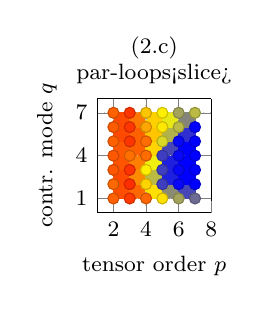
\begin{tikzpicture}
\begin{axis}
[
width=0.25\textwidth,
height=0.25\textwidth,
style={font=\footnotesize},
grid=major,
grid style={dotted},
align=center,
xlabel={tensor order $p$},
ylabel={contr. mode $q$},
title={(2.c)\\\tss{par-loops<slice>}}, %  ompfor<slice>, symmetric, row-major
title style={yshift=-1ex,},
scaled ticks=false,
zlabel={GFlops},
view={0}{90}, 
ytick={1,4,7,10},
xtick={2,4,6,8},
xmin=1, xmax=8,
ymin=0, ymax=8,
try min ticks=8,
zmin=0, zmax=55,
point meta min=0, point meta max=55,
colormap/hot, 
samples=50,
]
\addplot3[contour filled={number=100},scatter,shader=flat,samples=50]
coordinates{

(2.000,1.000,41.029) (2.000,2.000,39.659) (2.000,3.000,42.072) (2.000,4.000,42.006) (2.000,5.000,41.210) (2.000,6.000,41.386) (2.000,7.000,41.078) 

(3.000,1.000,46.531) (3.000,2.000,48.387) (3.000,3.000,47.302) (3.000,4.000,38.512) (3.000,5.000,46.947) (3.000,6.000,46.769) (3.000,7.000,47.158) 

(4.000,1.000,40.145) (4.000,2.000,24.201) (4.000,3.000,20.816) (4.000,4.000,39.260) (4.000,5.000,39.224) (4.000,6.000,30.906) (4.000,7.000,26.495) 

(5.000,1.000,22.729) (5.000,2.000,4.696) (5.000,3.000,4.643) (5.000,4.000,4.686) (5.000,5.000,15.500) (5.000,6.000,21.816) (5.000,7.000,20.604) 

(6.000,1.000,12.019) (6.000,2.000,0.574) (6.000,3.000,0.569) (6.000,4.000,0.561) (6.000,5.000,0.567) (6.000,6.000,13.543) (6.000,7.000,11.584) 

(7.000,1.000,8.162) (7.000,2.000,0.080) (7.000,3.000,0.070) (7.000,4.000,0.071) (7.000,5.000,0.071) (7.000,6.000,0.071) (7.000,7.000,13.531) 



};
\end{axis}
\end{tikzpicture}
\hfill
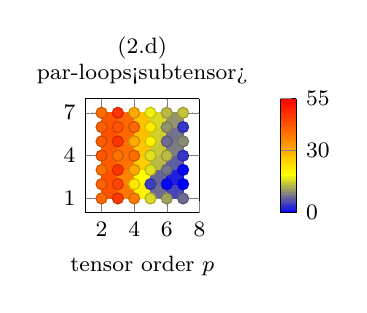
\begin{tikzpicture}
\begin{axis}
[
width=0.25\textwidth,
height=0.25\textwidth,
style={font=\footnotesize},
grid=major,
grid style={dotted},
align=center,
xlabel={tensor order $p$},
%ylabel={contr. mode (q)},
title={(2.d)\\\tss{par-loops<subtensor>}}, %  ompfor<subtensor>, symmetric, row-major
title style={yshift=-1ex,},
scaled ticks=false,
zlabel={GFlops},
view={0}{90}, 
%view={-45}{45}, 
ytick={1,4,7,10},
xtick={2,4,6,8},
xmin=1, xmax=8,
ymin=0, ymax=8,
try min ticks=8,
zmin=0, zmax=55,
point meta min=0, point meta max=55,
colormap/hot, 
samples=50,
colorbar sampled,
colorbar/width=0.2cm,
colorbar style={
point meta min=0, point meta max=55,
samples=50,
font=\footnotesize,
ytick={0,30,55},
yticklabels={0,30,55},
%title={\scriptsize Gflops},
%ylabel={\scriptsize Gflops},
}
]
\addplot3[contour filled={number=100},scatter,shader=flat,samples=50]
coordinates{

(2.000,1.000,39.925) (2.000,2.000,40.794) (2.000,3.000,38.666) (2.000,4.000,42.126) (2.000,5.000,41.384) (2.000,6.000,40.815) (2.000,7.000,39.521) 

(3.000,1.000,46.511) (3.000,2.000,44.987) (3.000,3.000,47.267) (3.000,4.000,38.092) (3.000,5.000,47.052) (3.000,6.000,42.441) (3.000,7.000,47.437) 

(4.000,1.000,37.335) (4.000,2.000,21.883) (4.000,3.000,30.773) (4.000,4.000,39.265) (4.000,5.000,30.464) (4.000,6.000,39.621) (4.000,7.000,30.520) 

(5.000,1.000,15.568) (5.000,2.000,4.650) (5.000,3.000,16.169) (5.000,4.000,16.207) (5.000,5.000,20.859) (5.000,6.000,21.162) (5.000,7.000,17.409) 

(6.000,1.000,11.911) (6.000,2.000,0.568) (6.000,3.000,8.276) (6.000,4.000,13.620) (6.000,5.000,7.950) (6.000,6.000,10.957) (6.000,7.000,13.327) 

(7.000,1.000,8.182) (7.000,2.000,0.080) (7.000,3.000,0.955) (7.000,4.000,4.006) (7.000,5.000,10.093) (7.000,6.000,4.165) (7.000,7.000,13.875) 

};
\end{axis}
\end{tikzpicture}